%----------------------------------------------------------------------
\documentclass[xcolor=svgnames]{beamer} %, handout
\usetheme{lined}
\usepackage{array}
\usepackage{amsmath}
\usepackage{amssymb}
\usepackage{amsthm}
\usepackage{bbm}
\usepackage[utf8]{inputenc}
\usepackage[T1]{fontenc}
\usepackage{cmbright}   
\usepackage{times}
\usepackage{geometry}
\usepackage[spanish]{babel}
\usepackage{multicol}
\usepackage{tcolorbox}

\usepackage{algorithm2e}

%\usepackage{psfrag}
\usepackage{graphicx}
\usepackage{color}
\usepackage{floatflt}
\usepackage{fancybox}
\usepackage{tabularx}
%\usepackage[all]{xy}
\usepackage{color}
\usepackage{siunitx} % para \degree
\usepackage{mathtools}
\usepackage{cancel}
\usepackage{tikz}
\usepackage{tikz-cd}
\usetikzlibrary{arrows,matrix,positioning}


\usetikzlibrary{positioning}
\usepackage{arydshln} %poder pone lineas punteadas en matrices




%\usepackage[most]{tcolorbox}


\theoremstyle{plain}
\newtheorem{definicion}{Definición}



\definecolor{redUnq}{rgb}{.7,.1,.1}
\definecolor{redUnq2}{rgb}{.5,.1,.3}

\mode<presentation>{
	%\usetheme{Boxes}
	%\usecolortheme[RGB={237,132,8}]{structure}
	%\usecolortheme[RGB={205,173,0}]{structure}
	\usecolortheme[RGB={100,10,10}]{structure}

	%\beamertemplateshadingbackground{SteelBlue!70}{Honeydew!10}
	%\usetheme{Warsaw}
	%\usecolortheme{default}
	\usetheme{Singapore}
	%\usetheme{Lined}
	%\usetheme[height=7mm]{Rochester} 
	\setbeamerfont{title}{shape=\bfseries,family=\rmfamily}
	%\usefonttheme[onlylarge]{structuresmallcapsserif}
	%\usefonttheme[onlysmall]{structurebold}
	\setbeamercolor{title}{fg=redUnq,bg=gray!40}
	\usefonttheme{professionalfonts}
	\setbeamercovered{highly dynamic}
	\setbeamercovered{transparent=10}
	\setbeamertemplate{navigation symbols}{}
	\colorlet{structure}{redUnq}

	\setbeamertemplate{frametitle}[default][left]
}

\definecolor{verzul}{rgb}{0, 0.5,0.5}

\renewcommand{\textbf}[1]{{\bfseries\textcolor{redUnq2}{#1}}}
\renewcommand{\emph}[1]{{\em\textcolor{redUnq2}{#1}}}

\setlength{\parindent}{0pt}
\theoremstyle{definition}
\newtheorem{ejem}{Ejemplo}
\newtheorem{defi}{Definición}
\newtheorem{ejer}{Ejercicio}
\newtheorem{prop}{Propiedad}
\newtheorem{lema}{Lema}
\newtheorem{teor}{Teorema}
\newtheorem{coro}{Corolario}

 

\newcommand{\Rset}{\mathbbmss{R}}
\newcommand{\Cset}{\mathbbmss{C}}
\newcommand{\PD}[2]{\frac{\partial #1}{\partial #2}}
\DeclareMathOperator{\tr}{tr}
\DeclareMathOperator{\adj}{adj}
\DeclareMathOperator{\rango}{rango}

\newenvironment{Boxedminipage}%
{\begin{Sbox}\begin{minipage}}%
{\end{minipage}\end{Sbox}\fbox{\TheSbox}}



\title{Métodos Numéricos - Clase 6}
  \logo{
\includegraphics[scale=0.25]{logoUnq} }
\author{Ulises Bussi- Javier Portillo}
%\institute{\scalebox{2}{\includegraphics[scale=0.1]{mdp02.jpg}}} %{Departamento de Ciencia y Tecnología\\ Universidad Nacional de Quilmes\\ }
\date{ $1^\circ$ cuatrimestre 2020} 


%%%%%%%%% Para que al comenzar una section aparezca el Contenido
%\AtBeginSection[]
%{
%  \begin{frame}
%    \frametitle{Contenidos de la Presentación}
%    \tableofcontents[currentsection]
%  \end{frame}
%}

\AtBeginSection[]
{
    \begin{frame}
        \frametitle{Ajustes de Curvas}
        \tableofcontents[currentsection]
    \end{frame}
}


\begin{document} 


\begin{frame} %\thispagestyle{empty}
	\titlepage
\end{frame}

\begin{frame}
\tableofcontents
\end{frame}


\section{Introducción Ajustes de curvas}

\begin{frame}
\frametitle{Modelado y Datos experimentales.}

\vspace{10pt}


\begin{tcolorbox}
\textbf{Predecir comportamiento}
Dado un conjunto de datos, predecir nuevos valores.
\end{tcolorbox} \vspace{20pt}

\textbf{¿Por qué?}
\pause
Es imposible medir todos los posibles valores de un modelo físico \pause $\rightarrow$ Modelamos y predecimos.


\end{frame}

\section{Regresión Lineal}

\begin{frame}{Regresión Lineal}
 Dado un conjunto de pares ordenados \visible<1->{ $\rightarrow$ Encontrar la recta que 	mejor   los representa.}
 \begin{center}
  \only<2>{ 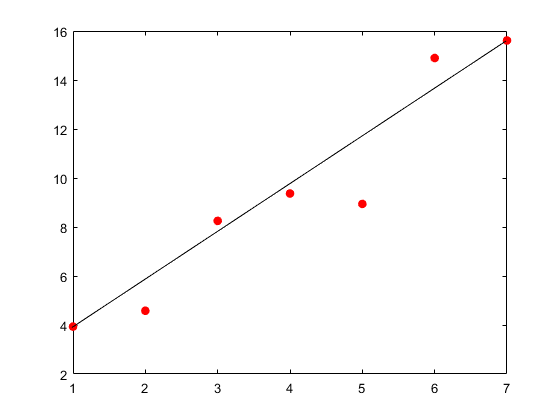
\includegraphics[scale=.4]{linFitManual/0.png}  }
  \only<3>{ 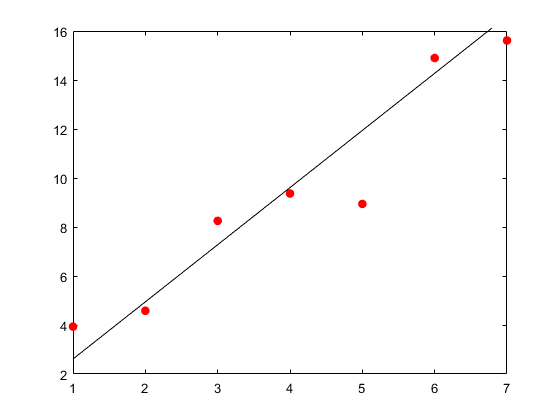
\includegraphics[scale=.4]{linFitManual/1.png} }
  \only<4->{ 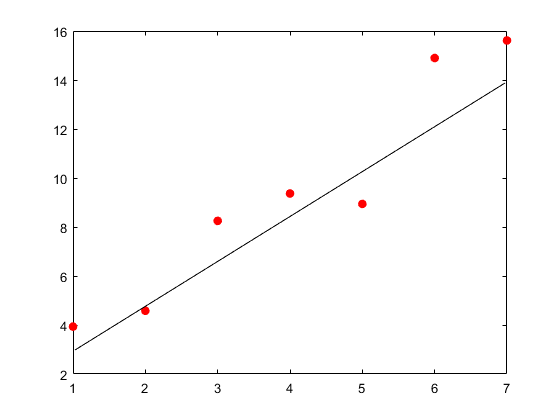
\includegraphics[scale=.4]{linFitManual/2.png} }

 \visible<5>{
 \begin{tcolorbox}\centering\textbf{Hay que definir un criterio}}
 \end{tcolorbox}
 \end{center}
\end{frame}

	
\begin{frame}{Regresión Lineal}
Podemos usar el Residual:\pause

Dado $\{x_i,y_i\}\ ,\ i =1,2,...,3$ y la recta $\hat y = a x+b$ el residual $S$ se calcula cómo:

$$ S = \sum_{i=1}^n y_i - \hat{y_i} = \sum_{i=1}^n y_i - (a* x_i +b) $$
\pause

E intentar minimizarlo $\rightarrow$ Encontrar $\{a,b\}$ para que el $"$ error $"$ sea lo más pequeño posible (S cercano a cero). 

\pause
\begin{tcolorbox}
\centering \textbf{No es buena idea!}
\end{tcolorbox}

\end{frame}


\begin{frame}{Regresión Lineal}
  \begin{minipage}{.6\linewidth}
    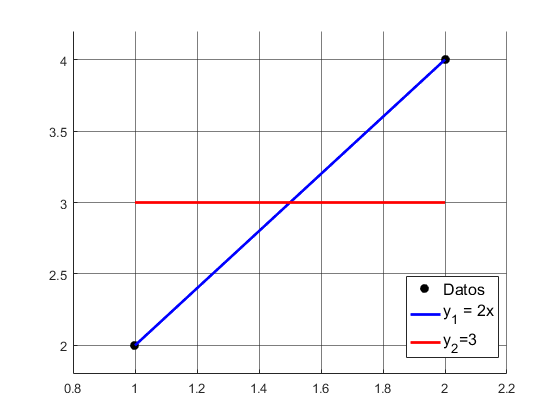
\includegraphics[width=\linewidth]{2pt_ResLin.png} 
  \end{minipage} \begin{minipage}{.35\linewidth}
    Para la recta $y_1$:
    $$ S = (2 - 2*1) + (4- 2*2) = 0$$
    
    Para la recta $y_2$:
    $$ S = (2- 3) + (4-3)  = 0$$
	  
  \end{minipage}
  
\end{frame}

\subsection{Cuadrados Mínimos}

\begin{frame}{Cuadrados Mínimos}
  \textbf{Propuesta:} minimizar 
  $$ S = \sum_{i=1}^n (y_i - \hat{y_i})^2 = \sum_{i=1}^n  \left[y_i - (a* x_i +b)\right]^2 $$ \pause
  
  O sea, encontrar $a$ y $b$ que hagan a $S$ lo más chico posible. \pause
  
  \textbf{¿Cómo?}
  Busco donde:\vspace{15pt}
  
  $\frac{\partial S}{\partial b} = 0$ $\leftarrow$ valor de $b$ que minimiza $S$\vspace{15pt}
  
  $\frac{\partial S}{\partial a} = 0$ $\leftarrow$ valor de $a$ que minimiza $S$

\end{frame}


\begin{frame}{Cuadrados Mínimos}
\begin{minipage}{.45\linewidth}
{\footnotesize

$$ \frac{\partial S}{\partial b} = \frac{\partial \sum_{i=1}^n\left[y_i - (a* x_i +b)\right]^2}{\partial b} $$

$$ \frac{\partial S}{\partial b} =  -2 \sum_{i=1}^n\left[y_i - (a* x_i +b)\right] = 0 $$

$$ \sum_{i=1}^n y_i - \sum_{i=1}^n (a*x_i) - \sum_{i=1}^n b = 0$$

$$\boxed{n {\color{red} b} + [\sum_{i=1}^n x_i] {\color{red} a} =  [\sum_{i=1}^n y_i] }$$
}
\end{minipage}\hspace{2pt} \vline\hspace{2pt} \begin{minipage}{.45\linewidth}
{\footnotesize

$$\frac{\partial S}{\partial a} = \frac{\partial \sum_{i=1}^n\left[y_i - (a* x_i +b)\right]^2}{\partial a} $$

$$\frac{\partial S}{\partial a} = -2\sum_{i=1}^n\left[(y_i - (a* x_i +b))(x_i) \right] = 0   $$

$$\sum_{i=1}^n x_i* y_i - \sum_{i=1}^n a*x_i^2- \sum_{i=1}^n x_i*b = 0 $$

$$\boxed{[\sum_{i=1}^n x_i]{\color{red}b} + [\sum_{i=1}^n x_i^2]{\color{red}a} = [\sum_{i=1}^n x_i*y_i]  } $$

}
\end{minipage} 
\end{frame}

\begin{frame}{Cuadrados mínimos}
Ahora tenemos este sistema de 2 ecuaciones con 2 incógnitas que se puede resolver:

\begin{tcolorbox}
$$a =  \frac{n \sum (x_i*y_i) -\sum x_i * \sum y_i}{n*\sum x_i^2 - (\sum x_i)^2}$$

$$b =  \bar y - a * \bar x  $$
\end{tcolorbox}
\end{frame}


\subsubsection{Ejemplo}
\begin{frame}{Ejemplo: cuadrados mínimos}
  Dado $x = [1, 2, 3, 4, 5, 6, 7]$ e $y = [3.93, 4.58, 8.25, 9.36,$ $ 8.94, 14.89, 15.61]$ encontrar la recta que mejor ajusta por cuadrados mínimos.
  
  \begin{minipage}{.3\linewidth}
    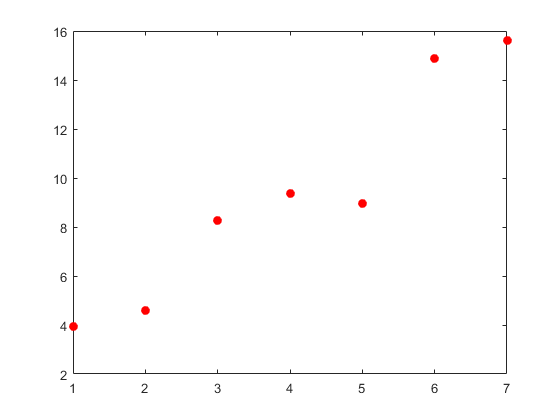
\includegraphics[width=\linewidth]{CuadradosMinimis/points.png} 
  \end{minipage}\vline \pause \begin{minipage}{.65\linewidth}
  Calculemos valores que necesitamos:
  \small
	\begin{minipage}{.45\linewidth}
	 $$\begin{array}{lll}
	   \sum x_i &=& 28 \\
	   \sum x_i*y_i &=& 318.59\\
	   \bar x = \frac{\sum x_i}{n} &=& 4
       \end{array}	  $$
	\end{minipage} 	\begin{minipage}{.45\linewidth}
	 $$\begin{array}{lll}
	   \sum y_i &=& 65.56 \\
	   \sum x_i^2 &=& 140\\
	   \bar y = \frac{\sum y_i}{n} &=& 9.37
       \end{array}	  $$
	\end{minipage} 	


  \end{minipage}
  
\end{frame}



\begin{frame}
  Dado $x = [1, 2, 3, 4, 5, 6, 7]$ e $y = [3.93, 4.58, 8.25, 9.36,$ $ 8.94, 14.89, 15.61]$ encontrar la recta que mejor ajusta por cuadrados mínimos.
  
  \begin{minipage}{.3\linewidth}
    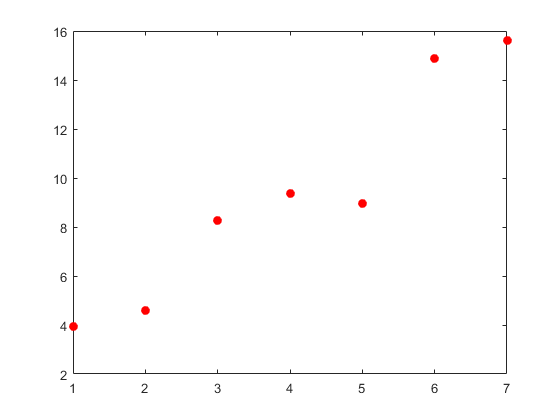
\includegraphics[width=\linewidth]{CuadradosMinimis/points.png} 
  \end{minipage}\vline \pause \begin{minipage}{.65\linewidth}
 	$$a = \frac{7*318.59 - 28*65.56} {7*140 - 28^2} = 2.0125$$

	$$b = 9.37 - {\color{red}2.0125} *4 = 1.32 $$
  \end{minipage} \pause
  
  \begin{tcolorbox}
   $$\hat y = 2.0125 x +1.32$$
  \end{tcolorbox}
\end{frame}


\begin{frame}{Ejemplo: cuadrados mínimos}
  Dado $x = [1, 2, 3, 4, 5, 6, 7]$ e $y = [3.93, 4.58, 8.25, 9.36,$ $ 8.94, 14.89, 15.61]$ encontrar la recta que mejor ajusta por cuadrados mínimos.
  
  \begin{center}
    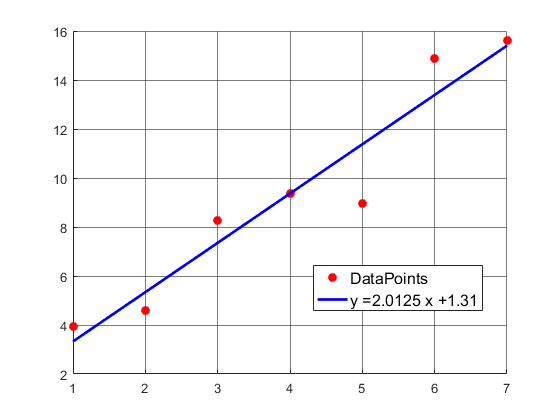
\includegraphics[width=.7\linewidth]{CuadradosMinimis/points_line.png} 
  \end{center}

\end{frame}

\subsubsection{Coeficiente de determinación}

\begin{frame}{Coeficiente de Determinación.}
Una vez realizado el ajuste podemos calcular:

  \begin{minipage}{.45\linewidth}
  
    El cuadrado de residual para todos los puntos:
    $$S_r = \sum_{i=1}^n (y_i - a*x_i -b)^2 $$
    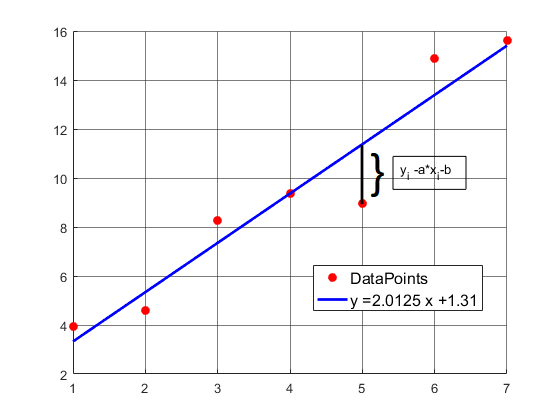
\includegraphics[width=\linewidth]{resid.png} 
  \end{minipage} \begin{minipage}{.45\linewidth}
	Y el residual respecto de la media:
	$$S_t = \sum_{i=1}^n (y_i - \bar y)^2 $$
    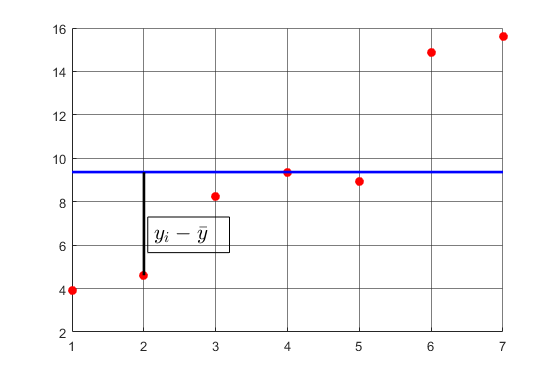
\includegraphics[width=\linewidth]{residm.png} 
  \end{minipage}

\end{frame}


\begin{frame}{Coeficiente de Determinación.}
Se llama coeficiente de determinación a la variable $r \in [0,1]$ que se calcula cómo:\pause

$$ r^2 = \frac{S_t - S_r}{S_t}$$

Nos dice cuanto mejor es ajustar la recta a los datos que simplemente usar el promedio.

\end{frame}

\section{Linealización y ajuste}


\begin{frame}{Relaciones no lineales.}
  Muchas veces, nos encontramos con relaciones No Lineales:\pause
  \begin{center}\begin{minipage}{.3\linewidth}
    $$y = a* e^{b*x}$$
    \center Modelo \\
    Exponencial
  \end{minipage}  \pause \begin{minipage}{.3\linewidth}
    $$y = a* x^{b}$$
    \center Modelo de \\
    potencia
  \end{minipage} \pause \begin{minipage}{.3\linewidth}
    $$y = a* \frac{x}{x+b}$$
    \center Modelo de \\
    crecimiento\\
    con saturación
  \end{minipage} \end{center}\pause
Es posible encontrar una transformación tal que se pueda expresar como un modelo lineal!
\end{frame}


\begin{frame}{Linealización y ajuste}
  Tomemos el modelo exponencial. Si trabajamos con el $\ln{y}$:
  \begin{minipage}{.45\linewidth}
    $$ \underbrace{\ln{y}}_{y^*} = \ln (a * e^{b*x}) $$
    $$y^* = \ln(a) + \ln(e^{b*x}) $$
    $$ y^* = \ln(a) + b*x $$
  \end{minipage} \begin{minipage}{.45\linewidth}
    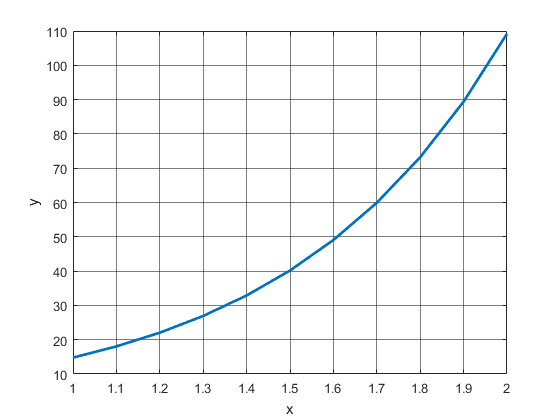
\includegraphics[scale=.3]{lin/exp.png} \\
    \visible<2->{ 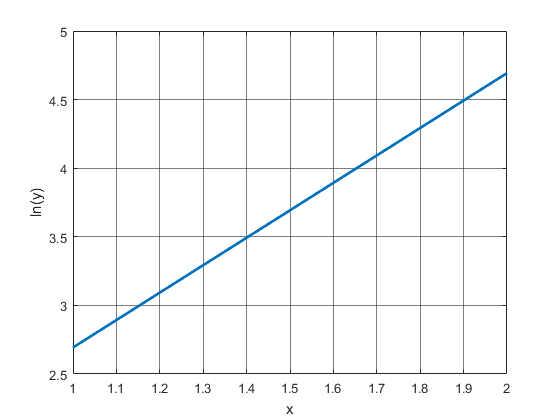
\includegraphics[scale=.3]{lin/exp_semilog.png}}
  \end{minipage}

\end{frame}





\begin{frame}{Linealización y ajuste}
  Tomemos el modelo de potencia. Si trabajamos con el $\ln{y}$:
  \begin{minipage}{.45\linewidth}
    $$ \underbrace{\ln{y}}_{y*} = \ln (a * x^b) $$
    $$y^* = \ln(a) + \ln(x^b) $$
    $$ y^* = \ln(a) + b*\underbrace{\ln (x)}_{x^*} $$
    $$ y^* = \ln(a) + b x^*$$
  \end{minipage} \begin{minipage}{.45\linewidth}
    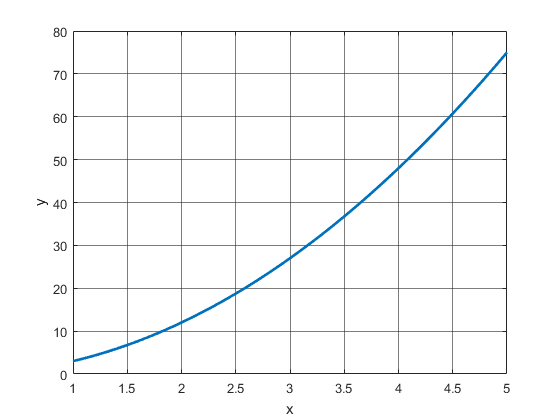
\includegraphics[scale=.3]{lin/pot.png} 
    
    \visible<2->{ 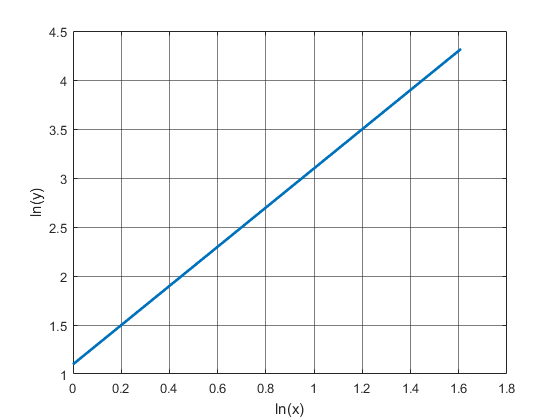
\includegraphics[scale=.3]{lin/pot_log.png}}
  \end{minipage}

\end{frame}

\section{Ajuste Polinomial}

\begin{frame}{Ajuste Polinomial}
  ¿Que sucede si quisieramos ajustar por ejemplo un polinomio de grado 2?\pause
  
  El mismo procedimiento de cuadrados mínimos podría ajustarse con un polinomio de la forma:
  $$ f(x) = a_0 + a_1 x + a_2 x^2$$
  
  A la hora de plantear el residual tendríamos:
  
  $$  S = \sum_{i=1}^n \left(y_i -a_0 -a_1*x_i -a_2 x_i^2\right)^2 $$
  
\end{frame}

\begin{frame}{Ajuste Polinomial}
  
  Debemos ahora derivar respecto a los 3 coeficientes para minimizar:
  $$\arraycolsep=1.4pt\def\arraystretch{3.2} \begin{array}{ccc}
  \frac{\partial S}{\partial a_0} &=& -2 \sum_{i=1}^n \left(y_i + a_0 +a_1 x_i +a_2 x_i^2\right)\\
  \frac{\partial S}{\partial a_1} &=& -2 \sum_{i=1}^n \left[\left(y_i + a_0 +a_1 x_i +a_2 x_i^2\right)x_i\right]\\
    \frac{\partial S}{\partial a_2} &=& -2 \sum_{i=1}^n \left[\left(y_i + a_0 +a_1 x_i +a_2 x_i^2\right)x_i^2\right]\\
\end{array}   $$
  
\end{frame}


\begin{frame}{Ajuste Polinomial}
  Operando y despejando como se realizó antes:
  
  $$\arraycolsep=1.4pt\def\arraystretch{2.2} \begin{array}{ccc}
  n*{\color{red}a_0}+{\color{red}a_1}*\sum x_i +{\color{red}a_2}* \sum x_i^2 &=& \sum y_i\\
  {\color{red}a_0}*\sum x_i+{\color{red}a_1}*\sum x_i^2 +{\color{red}a_2}* \sum x_i^3 &=& \sum y_i*x_i\\
  {\color{red}a_0}*\sum x_i^2+{\color{red}a_1}*\sum x_i^3 +{\color{red}a_2}* \sum x_i^4 &=& \sum y_i*x_i^2
\end{array}   $$\pause

\begin{center}
\begin{tcolorbox} \textbf{Un sistema de 3 ecuaciones con 3 incógnitas!!!} \end{tcolorbox}
\end{center}

\end{frame}

\begin{frame}{Ajuste Polinomial}
 En general, este método puede aplicarse a:
 \begin{itemize}
 \item sistemas con varias variables: $ S = \sum_{i=1}^n z_i- a_0 -a_1*x_i -a_2*y_i$
 \item sistemas no lineales:  $ S = \sum_{i=1}^n y_i- f(x_i)$
 \end{itemize}\pause
 En el último caso hay que tener cuidado, el problema puede convertirse en un sistema de ecuaciones no lineal.
\end{frame}


\section{Interpolación Polinómica}

\begin{frame}{Interpolación Polinómica}
  En general, si queremos predecir valores intermedios a valores dados, proponemos interpolar.  \pause

  \begin{tcolorbox}Aproximar el valor utilizando los valores conocidos.\end{tcolorbox} \pause


  Para un conjuntos de $n$ puntos existe un único polinomio de orden $n-1$ que pase por todos esos puntos.

\end{frame}

\begin{frame}{Interpolación Polinómica}
\small  
  Supongamos que tenemos 3 puntos conocidos $(x_i,y_i)$.


  Si queremos ajustar una parábola tenemos que buscar los 3 coeficientes $a_0,a_1,a_2$ que cumplen 
  $$ a_0 + a_1*x_i+ a_2*x_i^2 = y_i ,\ \forall i \in [1,2,3]$$\pause

  Es posible llevar esto a la forma matricial:
  $$\begin{bmatrix}
      x_1^2 & x_1 & 1 \\
      x_2^2 & x_2 & 1 \\
      x_3^2 & x_3 & 1 \\
    \end{bmatrix} \begin{bmatrix}
      a_2\\
      a_1\\
      a_0
    \end{bmatrix} = \begin{bmatrix}
      y_1\\
      y_2\\
      y_3
    \end{bmatrix}$$
  Esta matriz $A$ se conoce como matriz de Vandermonde. y son conocidas por ser muy mal condicionadas. \pause $\rightarrow$ El sistema será muy sensible.\pause

  \begin{tcolorbox}
    Se puede usar esta solución pero no es aconsejable
  \end{tcolorbox}
\end{frame}


\subsection{Interpolación de Newton}

\begin{frame}{Interpolación de Newton}
  Si queremos interpolar utilizando 2 puntos, los unimos con una recta y buscamos el valor que nos interesa relacionando las pendientes:
  
  \begin{minipage}{.45\linewidth}
  $$ \frac{f(x) - y_1}{x-x_1}  = \frac{y_2-y_1}{x_2-x_1} $$
  \visible<2->{Despejando:
  \begin{tcolorbox}\vspace{-7pt}
    $$ f(x) = y_1 + \frac{y_2-y_1}{x_2-x_1}(x-x_1)$$
    Polinomio interpolador de Newton de grado 1
  \end{tcolorbox}}  
  \end{minipage}\vline \begin{minipage}{.45\linewidth}
    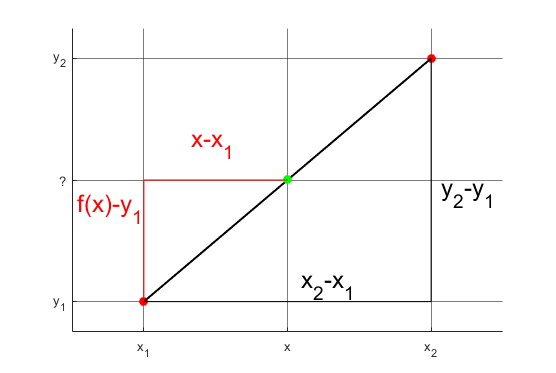
\includegraphics[width=\linewidth]{triangulosSemejantes.png} 
  \end{minipage}

\end{frame}




\begin{frame}{Interpolación de Newton}
  Si queremos interpolar utilizando 3 puntos proponemos el polinomio de grado 3:
  $$ f(x) = b_0 + b_1(x-x_1) + b_2(x-x_1)(x-x_2)  $$ 
  Si reemplazamos por los puntos conocidos tendremos: \pause
  $$ f(x_1) = b_0 + b_1\underbrace{(x_1-x_1)}_{0} + b_2\underbrace{(x_1-x_1)}_{0}(x_1-x_2) = b_0$$
  Con lo que $\boxed{ b_0 = f(x_1) = y_1}$

\end{frame}


\begin{frame}{Interpolación de Newton}
  Si queremos interpolar utilizando 3 puntos proponemos el polinomio de grado 3:
  $$ f(x) = b_0 + b_1(x-x_1) + b_2(x-x_1)(x-x_2)  $$ 
  Si reemplazamos por los puntos conocidos tendremos: \pause
  $$ f(x_2) = b_0 + b_1 (x_2-x_1) + b_2(x_2-x_1)\underbrace{(x_2-x_2)}_{0}$$
  con lo que si a $f(x_2)$ le restamos $b_0$ y dividimos por $(x_2-x_1)$:\pause
  
  $$\boxed{b_1  = \frac{f(x_2) -y_1}{x_2-x_1} = \frac{y_2-y_1}{x_2-x_1}}$$

\end{frame}

\begin{frame}{Interpolación de Newton}
  Por último:
  $$f(x_3) = b_0 + b_1(x_3-x_1) + b_2(x_3-x_1)(x_3-x_2) $$
  Restando $b_0$, dividiendo por $(x_3-x_1)$:\pause
  $$\frac{f(x_3) -b_0}{x_3-x_1} = b_1 +b_2(x_3-x_2) $$
  Si restamos el valor hallado de $b_1$ y dividimos por $(x_3-x_2)$:\pause
  
  \begin{minipage}{.45\linewidth}
      $$ \frac{\frac{f(x_3) -b_0}{x_3-x_1} - b_1}{x_3-x_2} = b_2$$
  \end{minipage}\pause$\rightarrow$\begin{minipage}{.45\linewidth}
      $$\boxed{ b_2 = \frac{\frac{y_3-y_1}{x_3-x_1} - \frac{y_2-y_1}{x_2-x_1} }{x_3-x_2} }$$
  \end{minipage}

\end{frame}

\begin{frame}{Interpolación de Newton}
  Resumiendo el de orden 2:
  $$ f(x) = b_0 + b_1(x-x_1) + b_2(x-x_1)(x-x_2)$$
  donde:
  
  \begin{minipage}{.45\linewidth}
    \begin{tcolorbox}
      $$b_0 = y_1$$
    \end{tcolorbox}
  \end{minipage}  \begin{minipage}{.45\linewidth}
    \begin{tcolorbox}
      $$b_1 = \frac{y_2 -y_1}{x_2-x_1}$$
    \end{tcolorbox}
  \end{minipage}
  \begin{center}
    \begin{minipage}{.6\linewidth}
      \begin{tcolorbox}
        $$b_2  = \frac{\frac{y_3-y_1}{x_3-x1} - \frac{y_3-y_2}{x_3-x_2}}{x_3-x_2}$$
      \end{tcolorbox}  
    \end{minipage}
  \end{center}

\end{frame}


\end{document}








